% Slide 31: Biological Inspiration
\begin{frame}{شبکه‌های عصبی مصنوعی}{\lr{Artificial Neural Networks - ANN}}
  \begin{itemize}
    \setlength{\itemsep}{10pt}
    \item \textbf{الهام‌گیری زیستی:}
    \begin{itemize}
      \item الهام گرفته از ساختار مغز انسان؛ یکی از قدرتمندترین سامانه‌های پردازش موازی و یادگیری جهان.
      \item شبکه‌ای متشکل از میلیاردها نورون به‌هم‌پیوسته که از طریق سیناپس‌ها سیگنال‌های الکتریکی و شیمیایی را مبادله می‌کنند.
    \end{itemize}
  \end{itemize}
  \vspace{0.15cm}
  \begin{center}
    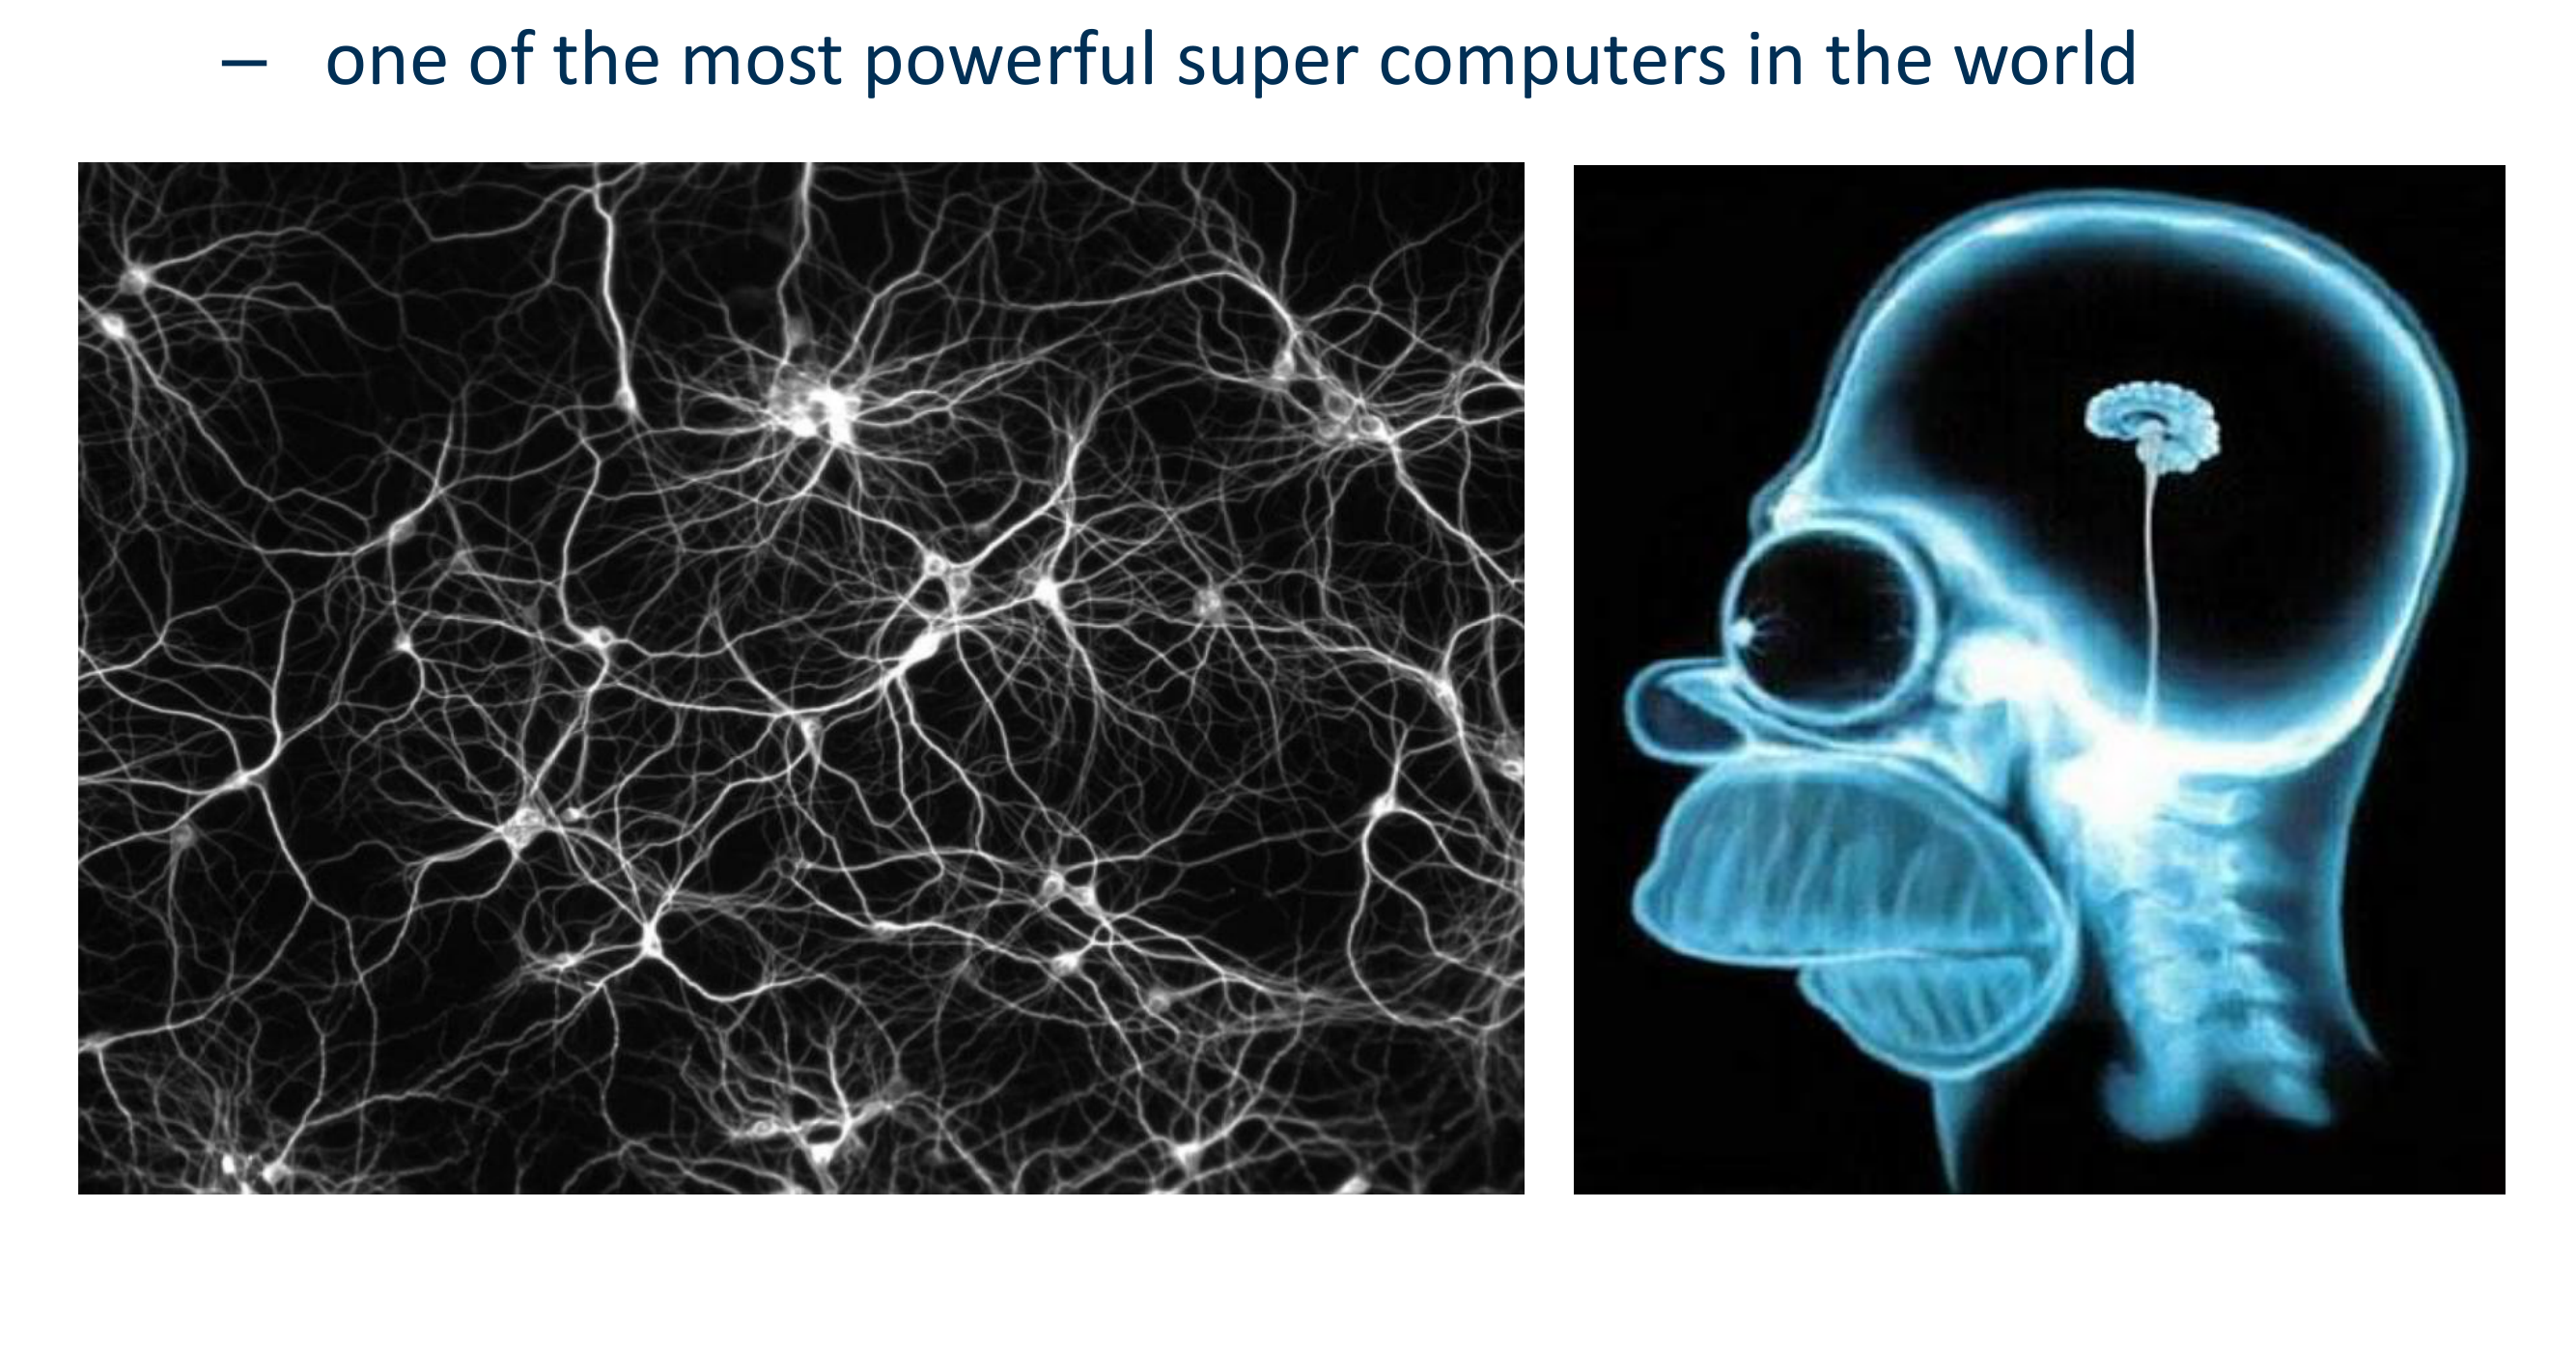
\includegraphics[width=0.88\textwidth,height=4.0cm,keepaspectratio]{images/slide31_neuron_comparison.png}
  \end{center}
\end{frame}

% Slide 32: Artificial Neuron Concept
\begin{frame}{برازش تابع بر داده‌های آموزش}{مفهوم پرسپترون اولیه}
  \begin{itemize}
    \item تابع مطلوب: خروجی $Y$ برابر با $1$ است اگر و تنها اگر \textbf{حداقل دو ورودی از سه ورودی} برابر با $1$ باشند.
  \end{itemize}
  \vspace{0.1cm}
  \begin{center}
    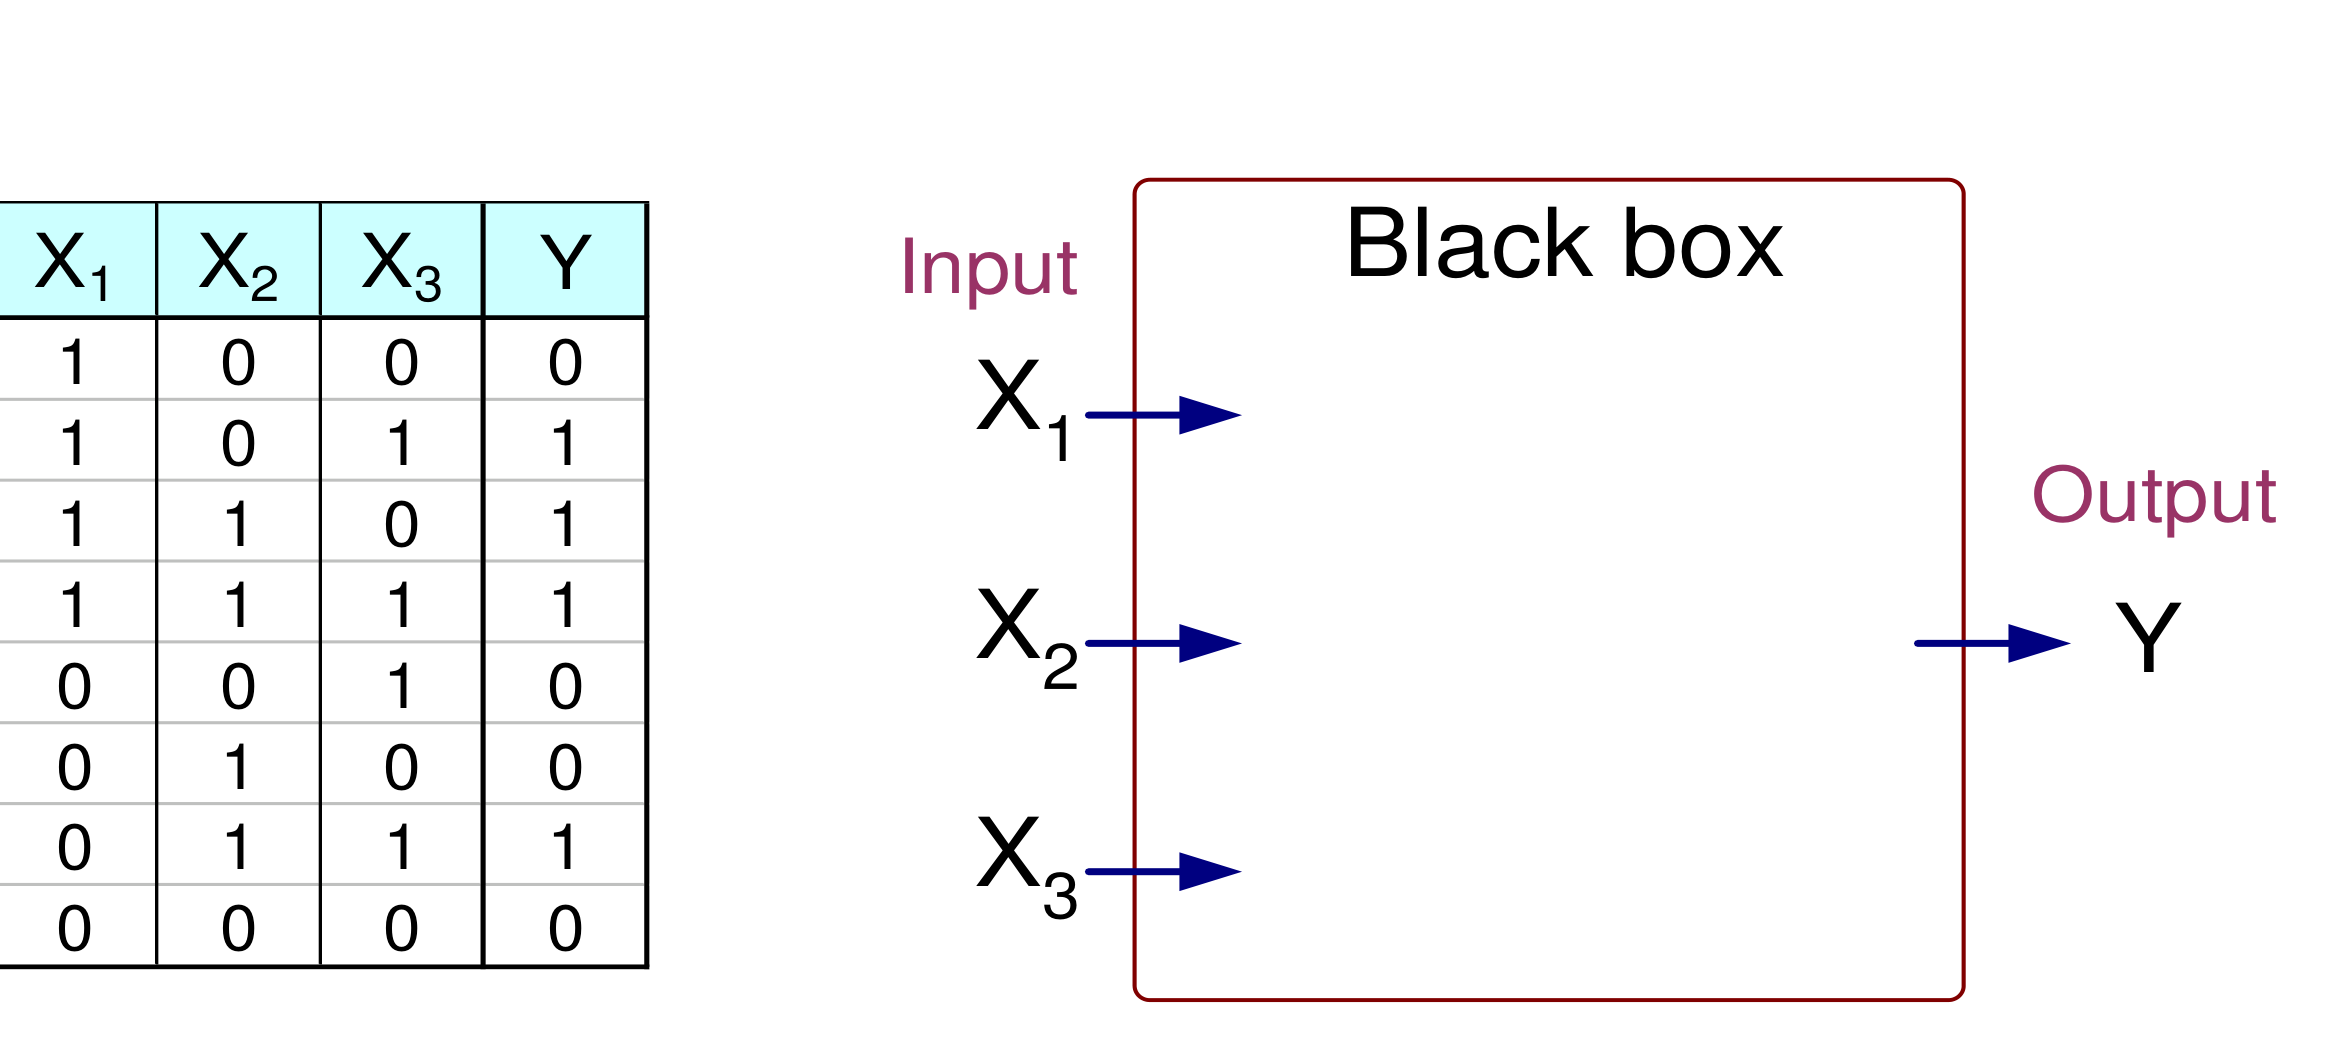
\includegraphics[width=0.85\textwidth,height=4.8cm,keepaspectratio]{images/slide32_perceptron_model.png}
  \end{center}
\end{frame}

% Slide 33: Perceptron Weights & Threshold
\begin{frame}{وزن‌دهی و آستانه تصمیم در پرسپترون}{مدل‌سازی ریاضی نورون}
  \begin{itemize}
    \item با تنظیم وزن‌های $w_i = 0.3$ و حد آستانه $t = 0.4$، معادله تصمیم به صورت زیر است:
  \end{itemize}
  \vspace{-0.1cm}
  \[
    Y = I(0.3 X_1 + 0.3 X_2 + 0.3 X_3 - 0.4 > 0)
  \]
  \vspace{-0.25cm}
  \begin{center}
    \small
    که در آن $I(z) = 1$ اگر شرط $z$ برقرار باشد، و در غیر این صورت $0$ است.
  \end{center}
  \vspace{0.1cm}
  \begin{center}
    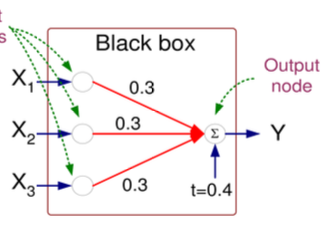
\includegraphics[height=3.7cm,keepaspectratio]{images/slide33_perceptron_black_box.png}
  \end{center}
\end{frame}

% Slide 34: General Perceptron Model
\begin{frame}{شبکه‌های عصبی مصنوعی}{مدل پرسپترون (\lr{Perceptron Model})}
  \begin{columns}[T]
    \begin{column}{0.55\textwidth}
      \begin{itemize}
        \setlength{\itemsep}{6pt}
        \item مدلی متشکل از گره‌های به‌هم‌پیوسته (نورون‌ها) و اتصالات وزن‌دار.
        \item گره خروجی، مجموع وزن‌دار مقادیر ورودی را طبق وزن یال‌ها محاسبه می‌نماید.
        \item \textbf{تصمیم طبقه‌بندی:} مقایسه گره خروجی با مقدار آستانه $t$:
      \end{itemize}
      \vspace{-0.1cm}
      \begin{latin}
        \[
          Y = I\left(\sum_{i=1}^k w_i X_i - t > 0\right)
        \]
      \end{latin}
    \end{column}
    \begin{column}{0.43\textwidth}
      \begin{center}
        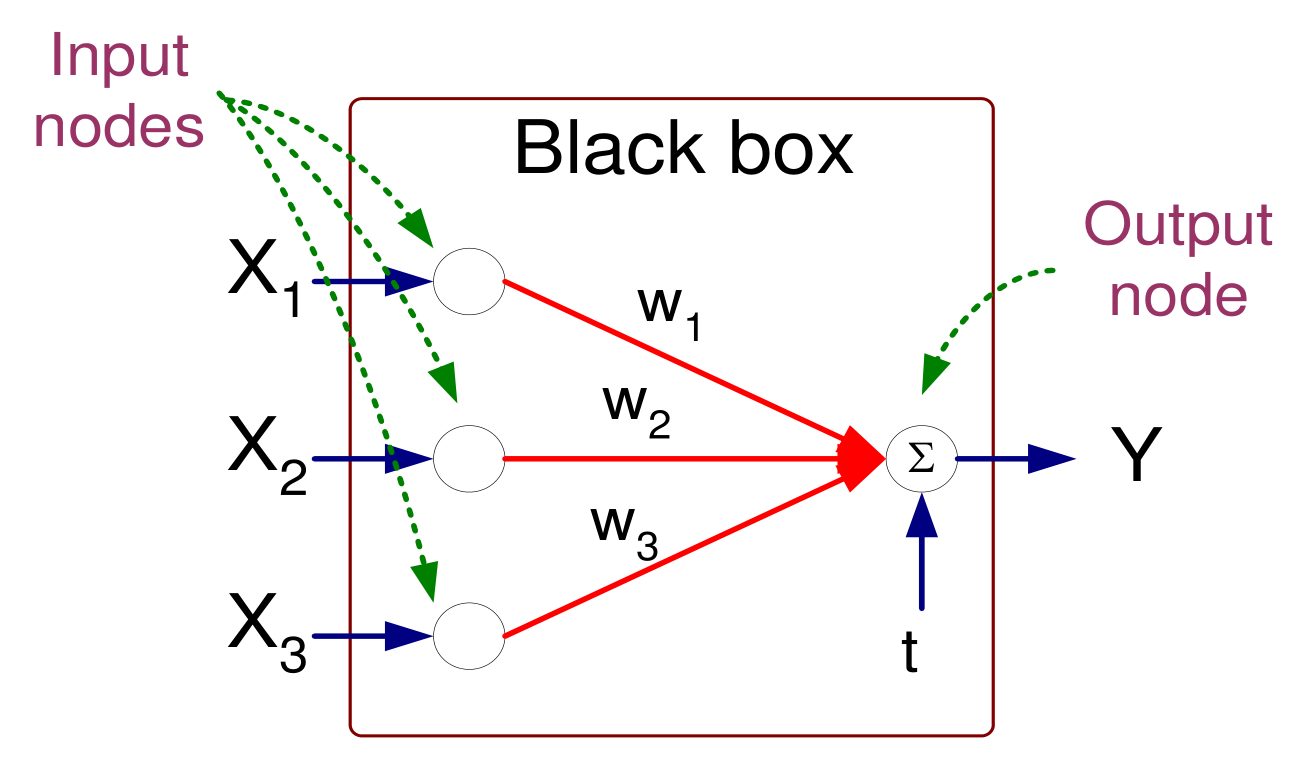
\includegraphics[width=\textwidth,height=3.8cm,keepaspectratio]{images/slide34_perceptron_diagram.png}
      \end{center}
    \end{column}
  \end{columns}
\end{frame}

% Slide 35: Multi-Layer Neural Networks
\begin{frame}{شبکه‌های عصبی چندلایه}{\lr{Multi-Layer Artificial Neural Networks (MLP)}}
  \begin{itemize}
    \item معماری شامل لایه ورودی (\lr{Input})، لایه‌های پنهان (\lr{Hidden Layers}) و لایه خروجی (\lr{Output}).
    \item \textbf{یادگیری در شبکه عصبی:} بهینه‌سازی و تنظیم وزن‌های اتصالات میان نورون‌ها است.
  \end{itemize}
  \vspace{0.1cm}
  \begin{center}
    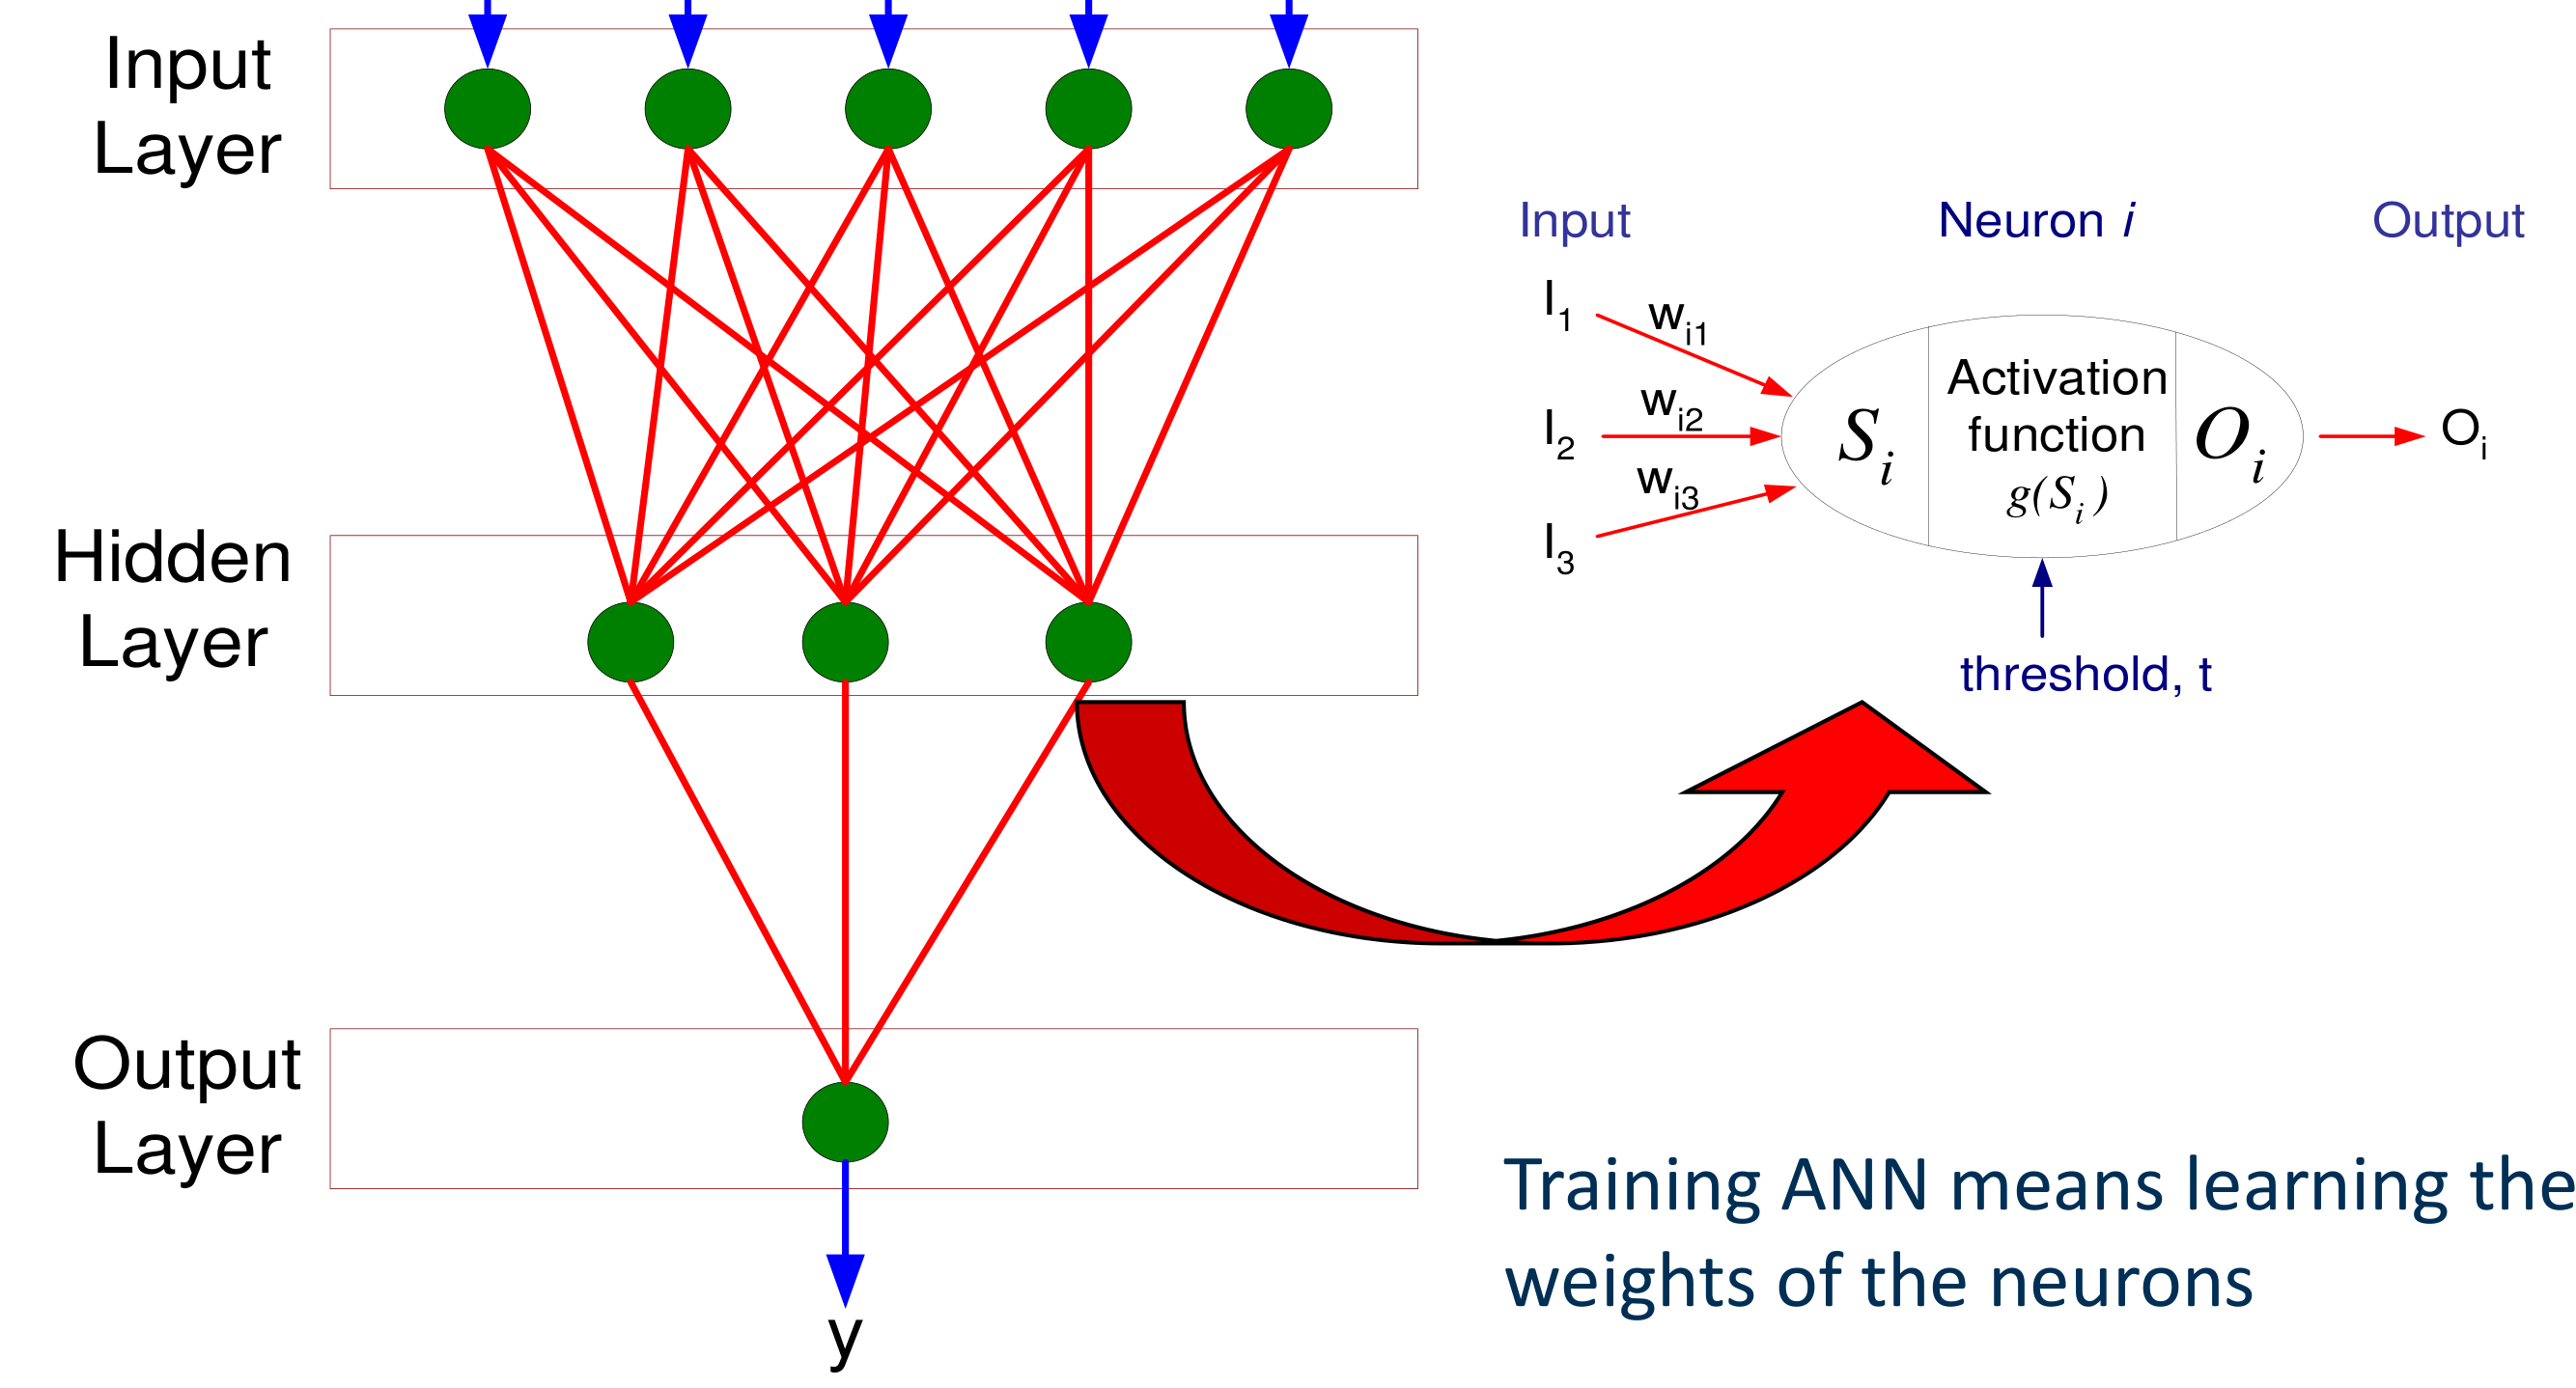
\includegraphics[width=0.90\textwidth,height=4.8cm,keepaspectratio]{images/slide35_mlp_architecture.png}
  \end{center}
\end{frame}

% Slide 36: Training Algorithm & Backpropagation
\begin{frame}{الگوریتم آموزش شبکه‌های عصبی}{\lr{Backpropagation Algorithm}}
  \begin{columns}[T]
    \begin{column}{0.58\textwidth}
      \begin{enumerate}
        \setlength{\itemsep}{4pt}
        \item \textbf{مقداردهی اولیه وزن‌ها} ($w_0, w_1, \dots, w_k$) به صورت تصادفی یا با مقادیر از پیش آموزش‌دیده.
        \item \textbf{تنظیم بازگشتی وزن‌ها} برای بیشترین تطابق با برچسب‌های واقعی آموزش:
        \begin{itemize}
          \setlength{\itemsep}{2pt}
          \item \textbf{تابع هدف:} کمینه‌سازی خطای مجموع مربعات (\lr{SSE}) به صورت $E = \sum_{i} [Y_i - f(w_i, X_i)]^2$
          \item استفاده از الگوریتم \textbf{پس‌انتشار خطا} (\lr{Backpropagation}) بر پایه گرادیان کاهشی.
          \item کنترل سرعت همگرایی با \textbf{نرخ یادگیری} (\lr{Learning Rate}).
        \end{itemize}
      \end{enumerate}
    \end{column}
    \begin{column}{0.40\textwidth}
      \begin{center}
        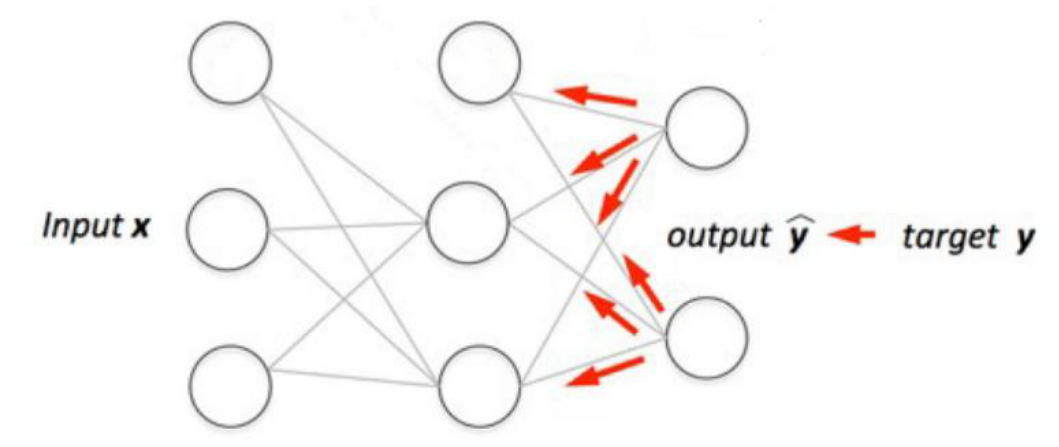
\includegraphics[width=\textwidth,height=2.5cm,keepaspectratio]{images/slide36_backprop_diagram.png}
      \end{center}
      \vspace{0.1cm}
      \begin{latin}
        \fcolorbox{codeborder}{codebg}{%
          \begin{minipage}{0.96\linewidth}
            \ttfamily\scriptsize
            \textbf{from} sklearn.neural\_network\\
            \hspace*{1em}\textbf{import} MLPClassifier\\[3pt]
            clf = MLPClassifier(\\
            \hspace*{1em}hidden\_layer\_sizes=(100,),\\
            \hspace*{1em}learning\_rate\_init=0.1)\\
            clf.fit(X\_train, y\_train)
          \end{minipage}%
        }
      \end{latin}
    \end{column}
  \end{columns}
\end{frame}

% Slide 37: Deep Learning Overview
\begin{frame}{مروری بر مدل‌های یادگیری عمیق}{\lr{Overview: Deep Learning Architectures}}
  \begin{itemize}
    \setlength{\itemsep}{12pt}
    \item \textbf{شبکه‌های عصبی پیچشی} (\lr{CNNs}): مدل‌های استاندارد در بینایی ماشین و پردازش تصویر.
    \item \textbf{مدل‌های زبانی از پیش آموزش‌دیده} (\lr{Pre-trained Models}): نظیر \lr{BERT} بر پایه ترنسفورمرها.
    \item \textbf{مدل‌های زایشی} (\lr{Generative Models}): مدل‌های تولید متن و تصویر نظیر \lr{GPT-3}، \lr{T5} و \lr{DALL-E}.
    \item \textbf{مدل‌های زبانی دستورپذیر} (\lr{Instruct Models}): سامانه‌های هوشمند تعاملی نظیر \lr{ChatGPT} مبتنی بر \lr{RLHF}.
  \end{itemize}
\end{frame}

% Slide 38: CNNs
\begin{frame}{شبکه‌های عصبی پیچشی}{\lr{Convolutional Neural Networks (CNNs)}}
  \begin{columns}[T]
    \begin{column}{0.50\textwidth}
      \begin{itemize}
        \setlength{\itemsep}{3pt}
        \item ابداع‌شده در حوزه بینایی ماشین (\lr{Computer Vision}).
        \item \textbf{ترکیب دو مؤلفه کلیدی:}
        \begin{enumerate}
          \setlength{\itemsep}{2pt}
          \item \textbf{یادگیری بازنمایی:} لایه‌های پیچش (\lr{Conv}) و ادغام (\lr{Pooling}).
          \item \textbf{سر پیش‌بینی} (\lr{Prediction Head}): لایه‌های کاملاً متصل (\lr{Dense}).
        \end{enumerate}
        \item کاهش تعداد متغیرها با لایه‌های پیچش و ادغام.
        \item \textbf{ظرفیت بالای مدل نیازمند:}
        \begin{itemize}
          \item حجم بالای داده‌های آموزش
          \item منابع سخت‌افزاری و زمان پردازش \lr{GPU} زیاد
        \end{itemize}
      \end{itemize}
    \end{column}
    \begin{column}{0.48\textwidth}
      \begin{center}
        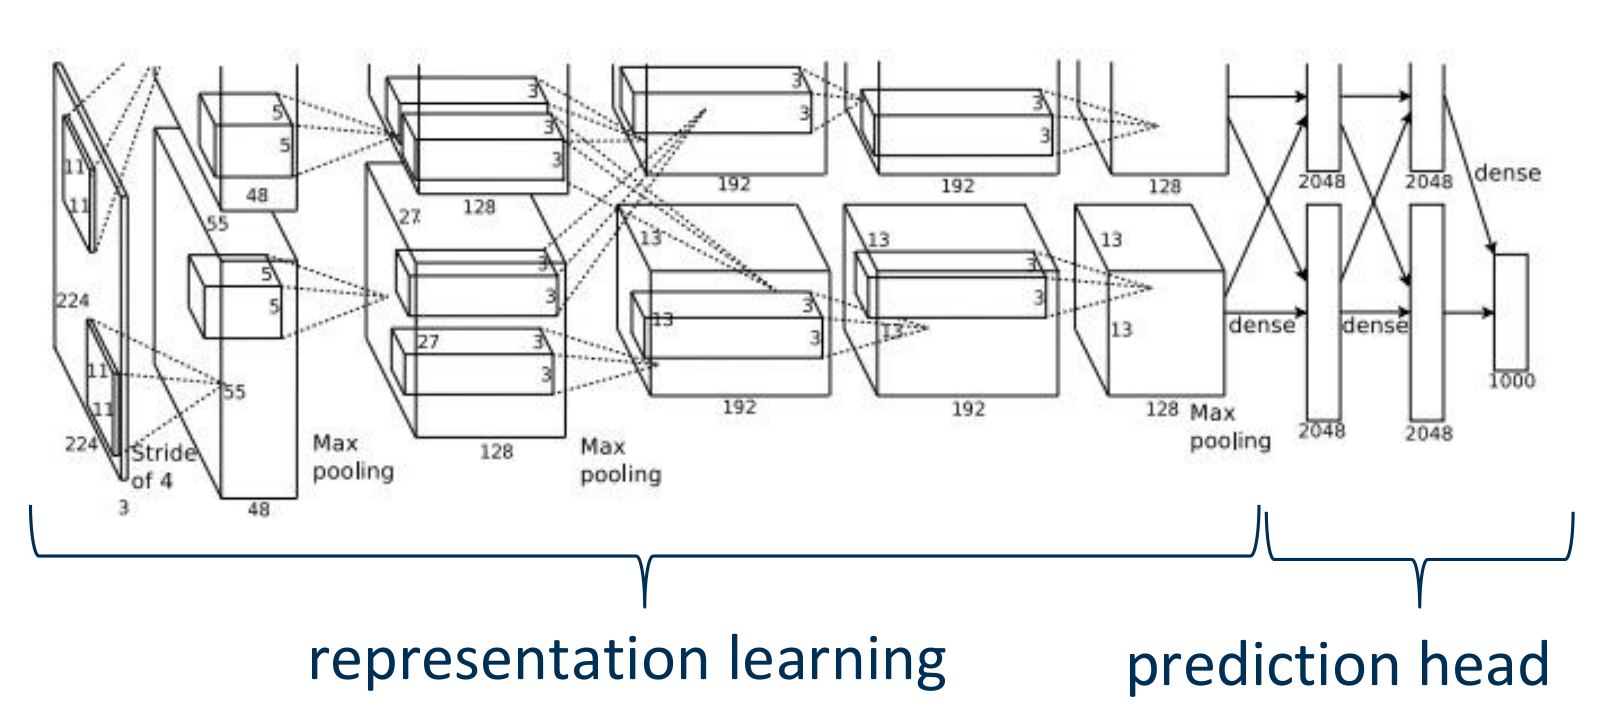
\includegraphics[width=\textwidth,height=2.1cm,keepaspectratio]{images/slide38_cnn_alexnet.png}\\[0.1cm]
        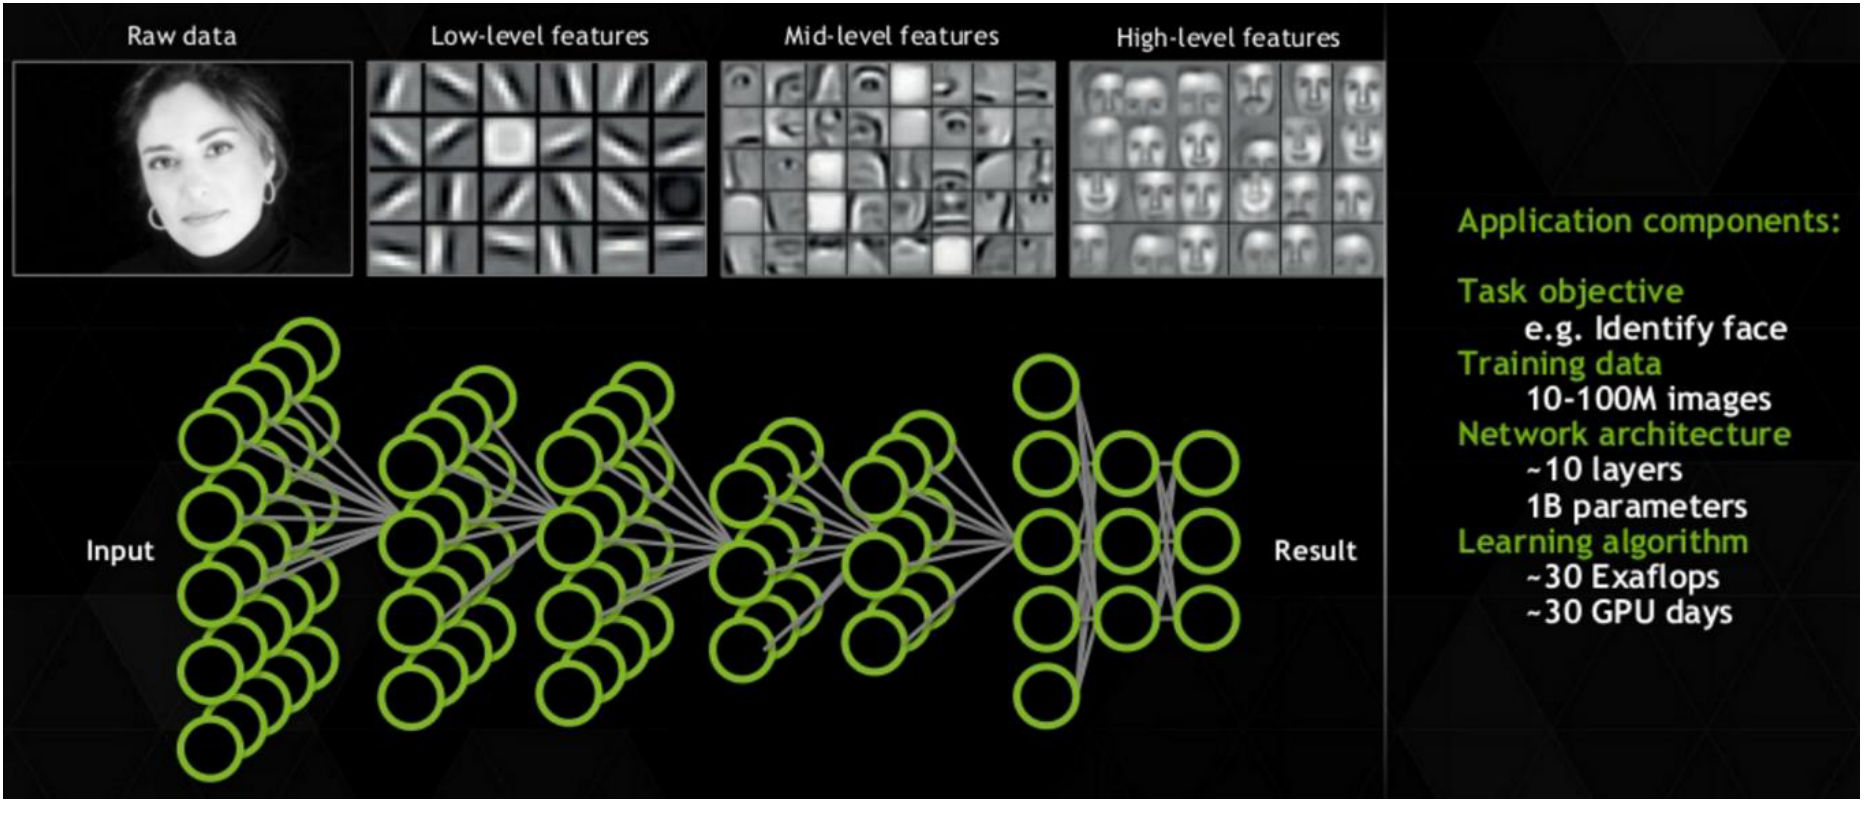
\includegraphics[width=\textwidth,height=2.6cm,keepaspectratio]{images/slide38_cnn_features.png}
      \end{center}
    \end{column}
  \end{columns}
\end{frame}

% Slide 39: Pre-Trained Language Models
\begin{frame}{مدل‌های زبانی از پیش‌آموزش‌دیده}{\lr{Pre-Trained Language Models (BERT)}}
  \begin{itemize}
    \setlength{\itemsep}{6pt}
    \item معرفی پارادایم نوین \textbf{پیش‌آموزش و سپس تنظیم دقیق} (\lr{Pre-training \& Fine-tuning}):
    \begin{itemize}
      \item پیش‌آموزش بر روی پیکره‌های متنی عظیم بدون نظارت انسانی.
      \item مدل \lr{BERT-base} با ۱۱۰ میلیون پارامتر و یادگیری بازنمایی دوجهته.
    \end{itemize}
    \item برتری قاطع بر تمامی روش‌های سنتی در اکثر آزمون‌های پردازش زبان طبیعی.
  \end{itemize}
  \vspace{0.05cm}
  \begin{center}
    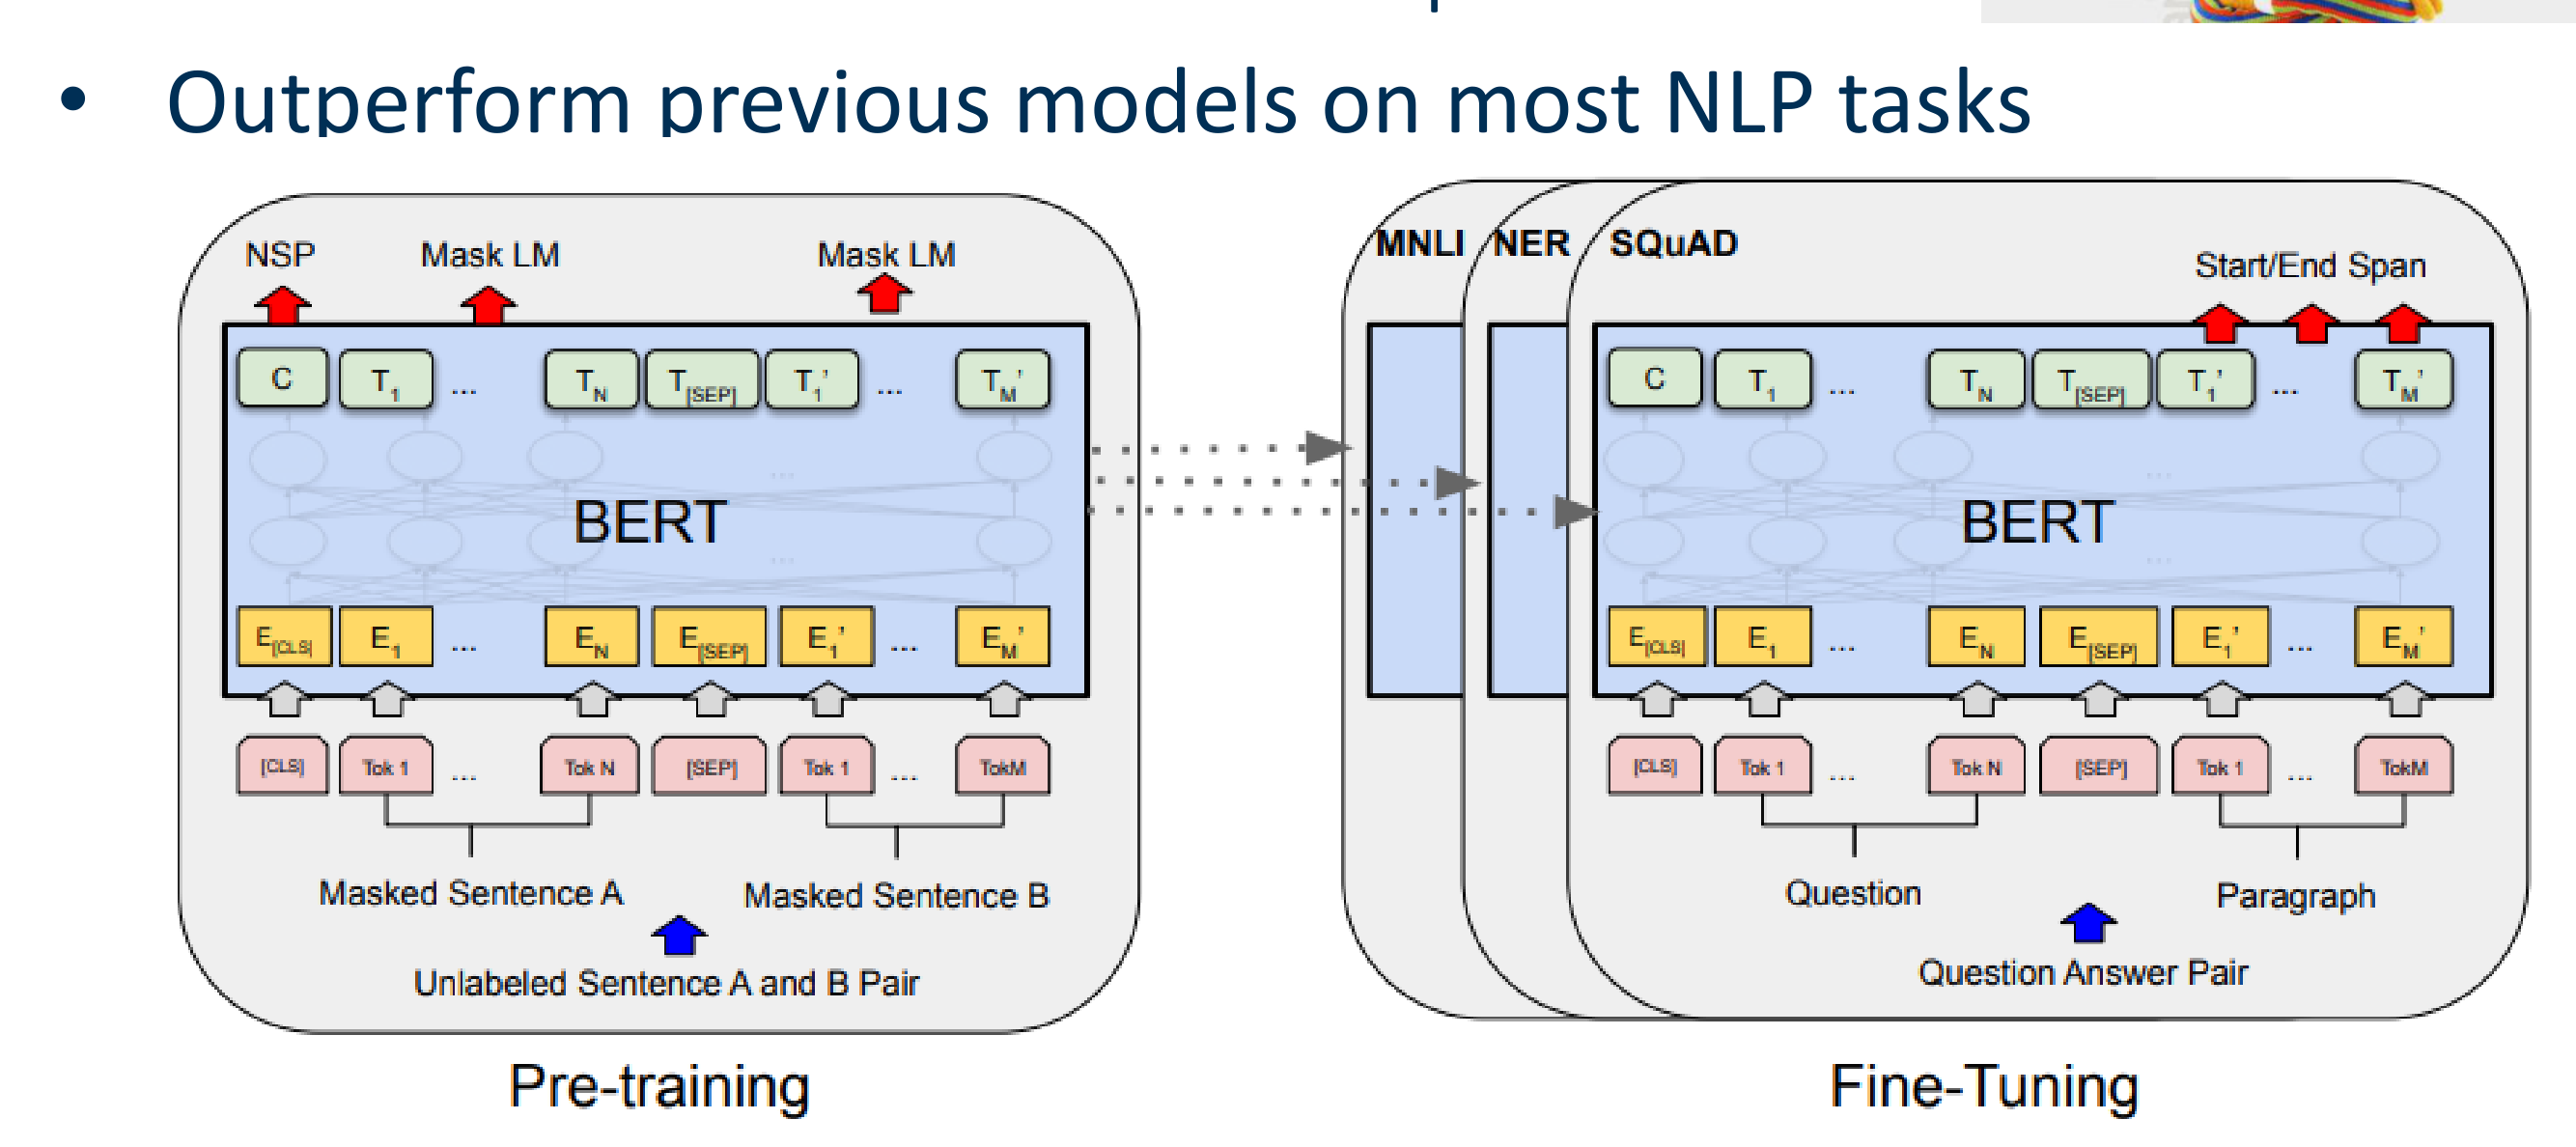
\includegraphics[width=0.88\textwidth,height=4.2cm,keepaspectratio]{images/slide39_bert_pretraining.png}
  \end{center}
\end{frame}

% Slide 40: Generative Models
\begin{frame}{مدل‌های زایشی}{\lr{Generative Models (Transformers, GPT, DALL-E)}}
  \begin{columns}[c]
    \begin{column}{0.60\textwidth}
      \begin{itemize}
        \setlength{\itemsep}{6pt}
        \item استفاده از معماری ترنسفورمر برای تولید متن یا تصویر بر پایه تعبیه توالی‌ها.
        \item \textbf{مدل‌های متنی:} \lr{GPT-3} و \lr{T5}.
        \item \textbf{مدل‌های تصویری:} \lr{DALL-E} و \lr{Stable~Diffusion}.
        \item پیش‌آموزش روی داده‌های عظیم (\lr{Web~crawls}، \lr{ImageNet}).
        \item مقیاس مدل‌ها: ۵ تا ۱۷۵ میلیارد پارامتر (دسترسی عمدتاً از طریق \lr{API}).
      \end{itemize}
    \end{column}
    \begin{column}{0.38\textwidth}
      \begin{center}
        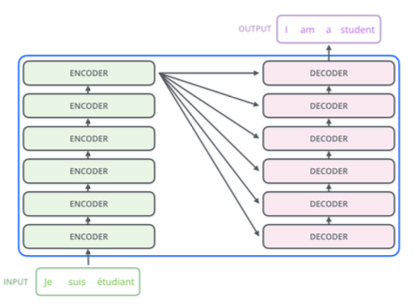
\includegraphics[width=\linewidth,height=4.8cm,keepaspectratio]{images/slide40_transformer_encoder_decoder.png}
      \end{center}
    \end{column}
  \end{columns}
\end{frame}

% Slide 41: Instruct Language Models
\begin{frame}{مدل‌های زبانی دستورپذیر}{\lr{Instruct Language Models \& RLHF}}
  \begin{columns}[c]
    \begin{column}{0.56\textwidth}
      \begin{itemize}
        \setlength{\itemsep}{6pt}
        \item پس از پیش‌آموزش روی متون عظیم، مدل‌های دستورپذیر با جفت‌های «دستور/پاسخ» تنظیم دقیق می‌شوند.
        \item عملکرد چندنمونه‌ای (\lr{Few-shot}) در گستره وسیعی از وظایف (\lr{BIG-bench}).
        \item \textbf{ظهور توانمندی‌های نوپدید:}
        \begin{itemize}
          \item مدل‌ها وظایفی را انجام می‌دهند که مستقیماً برای آن‌ها آموزش ندیده‌اند (\mbox{\lr{Emergent Abilities}}).
        \end{itemize}
        \item طراحی اعلان (\lr{Prompt Design}) و یادگیری درون‌متنی عملکرد را تعیین می‌کنند.
      \end{itemize}
    \end{column}
    \begin{column}{0.42\textwidth}
      \begin{center}
        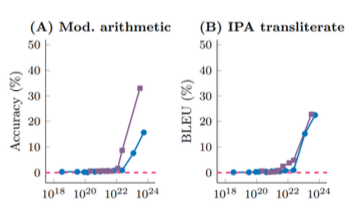
\includegraphics[width=\linewidth,height=4.8cm,keepaspectratio]{images/slide41_emergent_abilities.png}
      \end{center}
    \end{column}
  \end{columns}
\end{frame}
